\documentclass{book}

\usepackage{fontspec} % used to import Calibri
\usepackage{anyfontsize} % used to adjust font size

% needed for inch and other length measurements
% to be recognized
\usepackage{calc}

% for colors and text effects as is hopefully obvious
\usepackage[dvipsnames]{xcolor}
\usepackage{soul}

% control over margins
\usepackage[margin=1in]{geometry}
\usepackage[strict]{changepage}

\usepackage{mathtools}
\usepackage{amsfonts}
\usepackage{bm}

\usepackage[scr=rsfso, scrscaled=.96]{mathalpha}

% This is how I'm getting the nice caligraphy font :(
\DeclareMathAlphabet{\eulerscr}{U}{eus}{m}{n}
\newcommand{\mathcalli}[1]{\text{\scalebox{1.11}{$\eulerscr{#1}$}}}


\usepackage{amssymb} % originally imported to get the proof square
\usepackage{xfrac}
\usepackage[overcommands]{overarrows} % Get my preferred vector arrows...
\usepackage{relsize}

% Just am using this to get a dashed line in a table...
% Also you apparently want this to be inactive if you aren't
% using it because it slows compilation.
\usepackage{arydshln} \ADLinactivate 
\newenvironment{allowTableDashes}{\ADLactivate}{\ADLinactivate}

\usepackage{graphicx}
\graphicspath{{./158_Images/}}

\usepackage{tikz}
   \usetikzlibrary{arrows.meta}
   \usetikzlibrary{graphs, graphs.standard}

\usepackage{quiver} %commutative diagrams






\usepackage[hidelinks]{hyperref}
\newcommand{\inLinkRap}[2]{{\color{blue}\hyperlink{#1}{\textit{#2}}}}







\newfontfamily{\calibri}{Calibri}
\setlength{\parindent}{0pt}
\definecolor{RawerSienna}{HTML}{945D27}

% ~~~~~~~~~~~~~~~~~~~~~~~~~~~~~~~~~~~~~~~~~~~~~~~~~~
%Arrow Commands:

% Thank you Bernard, gernot, and Sigur who I copied this from:
% https://tex.stackexchange.com/questions/364096/command-for-longhookrightarrow
\renewcommand{\hookrightarrow}{\lhook\joinrel\rightarrow}
\renewcommand{\hookleftarrow}{\leftarrow\joinrel\rhook}
\newcommand{\hooklongrightarrow}{\lhook\joinrel\longrightarrow}
\newcommand{\hooklongleftarrow}{\longleftarrow\joinrel\rhook}
\newcommand{\hookxlongrightarrow}[2][]{\lhook\joinrel\xrightarrow[#1]{#2}}
\newcommand{\hookxlongleftarrow}[2][]{\xleftarrow[#1]{#2}\joinrel\rhook}

% Thank you egreg who I copied from:
% https://tex.stackexchange.com/questions/260554/two-headed-version-of-xrightarrow
\newcommand{\longrightarrowdbl}{\longrightarrow\mathrel{\mkern-14mu}\rightarrow}
\newcommand{\longleftarrowdbl}{\leftarrow\mathrel{\mkern-14mu}\longleftarrow}

\newcommand{\xrightarrowdbl}[2][]{%
  \xrightarrow[#1]{#2}\mathrel{\mkern-14mu}\rightarrow
}
\newcommand{\xleftarrowdbl}[2][]{%
  \leftarrow\mathrel{\mkern-14mu}\xleftarrow[#1]{#2}
}

\newcommand{\mRoman}[1]{%
   \textrm{\MakeUppercase{\romannumeral #1}}%
}



% ~~~~~~~~~~~~~~~~~~~~~~~~~~~~~~~~~~~~~~~~~~~~~~~~~~

\newcommand{\hOne}{%
   \color{Black}%
   \fontsize{14}{16}\selectfont%
}
\newcommand{\hTwo}{%
\color{Black}%
   \fontsize{13}{15}\selectfont%
}
% \newcommand{\scratchWork}{%
%    \color{PineGreen!85!Orange}
%    \fontsize{12}{14}\selectfont%
% }
\newcommand{\hThree}{%
   \color{Black}%
   \fontsize{12}{14}\selectfont%
}
\newcommand{\myComment}{%
   \color{RawerSienna}%
   \fontsize{12}{14}\selectfont%
}
\newcommand{\pracOne}{
   \color{BrickRed}%
   \fontsize{13}{15}\selectfont%
}
\newcommand{\pracTwo}{
   \color{Orange}%
   \fontsize{12}{14}\selectfont%
}
\newcommand{\why}{%
   \color{Orange}%
   \fontsize{12}{14}\selectfont%
	Why:
}
\newcommand{\exOne}{%
   \color{Purple}%
   \fontsize{14}{16}\selectfont%
}
\newcommand{\exTwo}{%
   \color{Purple}%
   \fontsize{13}{15}\selectfont%
}
\newcommand{\exThree}{%
   \color{Purple}%
   \fontsize{12}{14}\selectfont%
}
\newcommand{\exP}{%
   \color{Purple}%
   \fontsize{12}{14}\selectfont%
}
\newcommand{\exTwoP}{%
   \color{RedViolet}%
   \fontsize{13}{15}\selectfont%
}
\newcommand{\exThreeP}{%
   \color{RedViolet}%
   \fontsize{12}{14}\selectfont%
}
\newcommand{\exFourP}{%
   \color{RedViolet}%
   \fontsize{11}{13}\selectfont%
}
\newcommand{\exPP}{%
   \color{RedViolet}%
   \fontsize{12}{14}\selectfont%
}
\newcommand{\exPPP}{%
   \color{VioletRed}%
   \fontsize{12}{14}\selectfont%
}

% Homework standard below (God the bloat in the header is absurd...)
% ~~~~~~~~~~~~~~~~~~~~~~~~~~~~~~~~~~~~~~~~~~~~~~~~
\newcommand{\Hstatement}{%
   \color{MidnightBlue!90!Black}%
   \fontsize{12}{13}\selectfont%
}
\newcommand{\HexOne}{%
   \color{Purple}%
   \fontsize{12}{13}\selectfont%
}
\newcommand{\HexTwoP}{%
   \color{RedViolet}%
   \fontsize{12}{13}\selectfont%
}
\newcommand{\HexPPP}{%
   \color{VioletRed}%
   \fontsize{11}{12}\selectfont%
}

% ~~~~~~~~~~~~~~~~~~~~~~~~~~~~~~~~~~~~~~~~~~~~~~~~

\newcommand{\cyPen}[1]{{\vphantom{.}\color{Cerulean}#1}}
\newcommand{\redPen}[1]{{\vphantom{.}\color{Red}#1}}

\newenvironment{myIndent}{%
   \begin{adjustwidth}{2.5em}{0em}%
}{%
   \end{adjustwidth}%
}

\newenvironment{myDindent}{%
   \begin{adjustwidth}{5em}{0em}%
}{%
   \end{adjustwidth}%
}

\newenvironment{myTindent}{%
   \begin{adjustwidth}{7.5em}{0em}%
}{%
   \end{adjustwidth}%
}

\newenvironment{myConstrict}{%
   \begin{adjustwidth}{2.5em}{2.5em}%
}{%
   \end{adjustwidth}%
}

\newcommand{\udefine}[1]{{%
   \setulcolor{Red}%
   \setul{0.14em}{0.07em}%
   \ul{#1}%
}}

\newcommand{\uprop}[1]{{%
   \setulcolor{Purple}%
   \setul{0.14em}{0.07em}%
   \ul{#1} 
}}

\newcommand{\blab}[1]{\textbf{#1}}
\newcommand{\blect}[1]{{\color{MidnightBlue}\textbf{#1}}}

\newcommand{\uuline}[2][.]{%
{\vphantom{a}\color{#1}%
\rlap{\rule[-0.18em]{\widthof{#2}}{0.06em}}%
\rlap{\rule[-0.32em]{\widthof{#2}}{0.06em}}}%
#2}

\newcommand{\pprime}{{\prime\prime}}
\newcommand{\suchthat}{ \hspace{0.3em}s.t.\hspace{0.3em}}
\newcommand{\rea}[1]{\mathrm{Re}(#1)}
\newcommand{\ima}[1]{\mathrm{Im}(#1)}
\newcommand{\comp}{\mathsf{C}}
\newcommand{\trans}{\mathsf{T}}
\newcommand{\myHS}{ \hspace{0.5em}}
\newcommand{\gap}{\phantom{2}}

\newcommand{\GenLin}{\ensuremath{\mathrm{GL}}}
\newcommand{\Cay}{\ensuremath{\mathrm{Cay}}}

\newcommand{\myId}{\mathrm{Id}}
\newcommand{\myIm}{\mathrm{im}}
\newcommand{\Obj}{\mathrm{Obj}}
\newcommand{\Hom}{\mathrm{Hom}}
\newcommand{\End}{\mathrm{End}}
\newcommand{\Aut}{\mathrm{Aut}}

\newcommand{\df}{\mathrm{d}}
\newcommand{\Df}{\mathrm{D}}

\newcommand{\mcateg}[1]{{\bm{\mathsf{#1}}}}

\newcommand{\mdeg}{\mathrm{mdeg}\phantom{.}}

\newcommand{\divides}{\mathop{\mid}}

\newcommand{\card}{\mathrm{card}}
\newcommand{\supp}{\mathrm{supp}}
\newcommand{\diam}{\mathrm{diam}}
\newcommand{\conv}{\mathrm{conv}}
\newcommand{\opnorm}{\mathrm{op}}
\newcommand{\loc}{\mathrm{loc}}
\newcommand{\sgn}{\mathrm{sgn}}
\newcommand{\acc}{\mathrm{acc}}

\newcommand{\mSpan}{\mathrm{span}}
\newcommand{\Interior}{\mathop{\mathrm{Int}}}

\newcommand{\mMat}[1]{\mathbf{#1}}

\newcommand{\NBV}{\ensuremath{\mathrm{NBV}}}
\newcommand{\Acc}{\mathrm{Acc}}
\newcommand{\BV}{\ensuremath{\mathrm{BV}}}
\newcommand{\Var}{\ensuremath{\mathrm{Var}}}

\newcommand{\Alt}{\mathrm{Alt}}
\newcommand{\Sym}{\mathrm{Sym}}

\newcommand{\weakst}{weak$^*$ }

\newcommand{\radtimes}{\mathop{\widehat{\times}}}

\newcommand{\mMod}[1]{\phantom{a}(\mathrel{\mathrm{mod}} #1)}
\newcommand{\Fun}{\mathrm{Fun}}
\newcommand{\act}{\mathrm{act}}
\newcommand{\Fix}{\mathrm{Fix}}
\newcommand{\Sub}{\mathrm{Sub}}
\newcommand{\Cl}{\mathrm{Cl}}
\newcommand{\GL}{\mathrm{GL}}
\newcommand{\SL}{\mathrm{SL}}
\newcommand{\core}{\mathrm{core}}
\newcommand{\Syl}{\mathrm{Syl}}
\newcommand{\Iso}{\mathrm{Iso}}
\newcommand{\Homeo}{\mathrm{Homeo}}
\newcommand{\Inn}{\mathrm{Inn}}


\DeclareMathOperator{\lcm}{lcm}
\DeclareMathOperator{\symdif}{\triangle}
\DeclareMathOperator{\Average}{Average}
\DeclareMathOperator*{\AverageAst}{Average}

% Thank you Gonzalo Medina and Moriambar who wrote this on stack exchange:
%https://tex.stackexchange.com/questions/74125/how-do-i-put-text-over-symbols%
\newcommand{\myequiv}[1]{\stackrel{\mathclap{\mbox{\footnotesize{$#1$}}}}{\equiv}}

% Thank you chs who wrote this on stack exchange:
%https://tex.stackexchange.com/questions/89821/how-to-draw-a-solid-colored-circle%
\newcommand{\filledcirc}[1][.]{\ensuremath{\hspace{0.05em}{\color{#1}\bullet}\mathllap{\circ}\hspace{0.05em}}}

%Thank you blerbl who wrote this on stack exchange:
%https://tex.stackexchange.com/questions/25348/latex-symbol-for-does-not-divide
\newcommand{\ndiv}{\hspace{-0.3em}\not|\hspace{0.35em}}

\newcommand{\mySepOne}[1][.]{%
   {\noindent\color{#1}{\rule{6.5in}{1mm}}}\\%
}
\newcommand{\mySepTwo}[1][.]{%
   {\noindent\color{#1}{\rule{6.5in}{0.5mm}}}\\%
}
\newcommand{\mySepThree}[1][.]{%
   {\noindent\color{#1}{\rule{6in}{0.25mm}}}\\%
}

\newenvironment{myClosureOne}[2][.]{%
   \color{#1}%
   \begin{tabular}{|p{#2in}|} \hline \\%
}{%
   \\ \hline \end{tabular}%
}

\newcommand{\retTwo}{\hfill\bigbreak}

\newcommand{\dispDate}[1]{{
   \color{Black}%
   \fontsize{20}{18}\selectfont%
   #1\retTwo
}}


\begin{document}
\setul{0.14em}{0.07em}
\calibri

\hTwo\dispDate{10/17/2025}

So for functional analysis I need some fixed point theorems that would normally have been taught in a topology class. But I've never taken an actual topology class. Hence, my goal for today is to prove those theorems. First, I will be taking notes from the paper \textit{Brouwer's Fixed Point Theorem} by Jasmine Katz. (See the \inLinkRap{bib citation 17}{17th entry} of the bibliography\dots)\retTwo

Katz defines a \udefine{convex body} in $\mathbb{R}^n$ to be a set $X \subseteq \mathbb{R}^n$ that is compact, convex, and has a nonempty interior (relative to the Euclidean topology of all of $\mathbb{R}^n$).\retTwo

Also, for $m \geq n \geq 1$ suppose we are given any $n + 1$ points $p_0, p_1 \ldots, p_n \in \mathbb{R}^m$ in general linear position (see my math 190b notes). Then we say the convex hull of those points (i.e. $\conv(p_0, p_1 \ldots, p_n)$) is an \udefine{$n$-simplex}. Recall from the notes I took before I dropped math 190b last Spring that all $n$-simplices are compact and homeomorphic to each other.\retTwo

Katz in particular denotes $\Delta_0^n \coloneqq \conv(e_1, \ldots, e_n, -\sum_{i=1}^n e_i)$ where $e_1, \ldots, e_n$ are\\ the standard basis vectors of $\mathbb{R}^n$. Also, Katz denotes $\Delta^n$ to be the \udefine{standard $n$-simplex}\\ $\conv(u_1, \ldots, u_{n+1})$ where $u_1, \ldots, u_{n+1}$ are the standard basis vectors of $\mathbb{R}^{n+1}$.\retTwo

\exTwo\ul{Proposition 3.2:} $\Delta_0^n$ is a convex body in $\mathbb{R}^n$.
\begin{myIndent}\exThreeP
	Proof:\\
	The only thing not trivial from the definition of $\Delta_0^n$ is that $\Delta_0^n$ has a nonempty interior. So to prove this, first define for each $k \in \mathbb{N}$ the $(k+1)$ by $(k+1)$ matrices:

	{\centering $A_k \coloneqq \begin{pmatrix}
		\begin{bmatrix} 1 & & \\ & \ddots & \\ & & 1 \end{bmatrix} & \begin{matrix} -1 \\ \vdots \\ -1 \end{matrix} \\ \begin{matrix} 1 & \cdots & 1 \end{matrix} & 1
	\end{pmatrix}$ and $B_k \coloneqq \begin{pmatrix}
		\begin{matrix} 0 \\ \vdots \\ 0 \end{matrix} & \begin{bmatrix} 1 & & \\ & \ddots & \\ & & 1 \end{bmatrix} \\ 1 & \begin{matrix} 1 & \cdots & 1 \end{matrix}
	\end{pmatrix}$ \retTwo\par}

	We can calculate the determinant of $A_k$ as follows:
	\begin{myIndent}\exPPP
		Clearly $\det(A_1) = \det(\left[ \begin{smallmatrix} 1 & -1 \\ 1 & 1 \end{smallmatrix}\right]) = 2$ and $\det(B_1) = \det(\left[ \begin{smallmatrix} 0 & 1 \\ 1 & 1 \end{smallmatrix}\right]) = -1$.\retTwo
		
		Meanwhile, by considering the Laplace expansions going along the top rows of $A_k$ and $B_k$ where $k > 1$, we get that:
		
		{\centering$\det(A_k) = \det(A_{k-1}) + (-1)^{k+3}\det(B_{k-1})$ and $\det(B_k) = -\det(B_{k-1})$\retTwo\par}

		From there it is easy to see that $\det(B_k) = (-1)^{k}$. And hence:
		
		{\centering\begin{tabular}{l}
			$\det(A_k) = \det(A_{k-1}) + (-1)^{(k + 3) + (k - 1)} = \det(A_{k-1}) + (-1)^{2(k + 1)}$\\
			$\phantom{\det(A_k) = \det(A_{k-1}) + (-1)^{(k + 3) + (k - 1)}} = \det(A_{k-1}) + 1$\\
			$\phantom{\det(A_k) = \det(A_{k-1}) + (-1)^{(k + 3) + (k - 1)}} = \det(A_{k-2}) + 2$\\
			$\phantom{\det(A_k) = \det(A_{k-1}) + (-1)^{(k + 3) + (k - 1)} = aaaaaaa} \vdots$\\
			$\phantom{\det(A_k) = \det(A_{k-1}) + (-1)^{(k + 3) + (k - 1)}} = \det(A_1) + (k-1) = k+1$\\
		\end{tabular}\retTwo\par}
	\end{myIndent}
	
	In particular, we now know that $A_n$ is invertible since it has nonzero determinant. And this is important because we can now say that $x = (x_1, \ldots, x_n) \in \Delta_0^n$ if and only if:
	
	{\centering\begin{tabular}{l}
		$f(x_1, \ldots, x_n) \coloneqq (A_n)^{-1}\left[\begin{smallmatrix} x_1 \\ \vdots \\ x_n \\ 1 \end{smallmatrix}\right] \in [0, \infty)^{n+1}$
	\end{tabular}\newpage\par}

	But $f$ is a continuous injection and $f(0) = (\frac{1}{n+1}, \ldots, \frac{1}{n+1})$ since:
	
	{\centering$0 = \sum_{i=1}^n \frac{1}{n + 1}e_i - \frac{1}{n+1}(\sum_{i=1}^n e_i)$.\retTwo\par}

	Hence, there must be some $\delta > 0$ such that $\|f(x) - f(0)\|_2 < \frac{1}{n+1}$ when $\|x\|_2 < \delta$. And in turn, the open ball of radius $\delta$ about $0$ is contained in $\Delta_0^n$. $\blacksquare$\retTwo
\end{myIndent}

\hTwo Katz defines a \udefine{ray} from $x_0 \in \mathbb{R}^n$ to be a set $\{x_0 + ty : t \geq 0\}$ where $y \in \mathbb{R}^n$ with $\|y\|_2 = 1$.\retTwo

\pracOne\mySepTwo
Here is a basic topology fact I somehow haven't proved before:\retTwo

\ul{Proposition:} Suppose $X$ is a topological space, $E \subseteq X$ is connected, and $A \subseteq X$ satisfies that $E \cap A \neq \emptyset$ and $E \cap A^\comp \neq \emptyset$. Then $E \cap \partial A \neq \emptyset$.
\begin{myIndent}\pracTwo
	Proof:\\
	Note that $\partial A = \overline{A} \cap \overline{A^\comp}$. So if $E \cap \partial A = \emptyset$, then this implies that $\overline{A} \cap E$ and $\overline{A^\comp} \cap E$\\ are two disjoint nonempty closed sets (in the subspace topology of $E$) whose union is\\ all of $E$. But this contradicts that $E$ is connected. $\blacksquare$
\end{myIndent}
\mySepTwo

\exTwo\ul{Lemma 3.6:} Suppose $X \subseteq \mathbb{R}^n$ is a convex body with $0 \in X^\circ$. Then every ray from $0$\\ intersects $\partial X$ exactly once.

\begin{myIndent}\exThreeP
	Proof:\\
	Fix $y \in \mathbb{R}^n$ such that $\|y\| = 1$ and let $f(t) = ty$. Then we want to show there is a unique $t_0 \geq 0$ such that $f(t_0) \in \partial X$. Fortunately, it's easy to see that $f(t)$ intercepts $\partial X$ at least once. After all, $f(0) \in X$. But at the same time, since $X$ is compact and thus bounded, we know that there is some $t^\prime > 0$ such that $f(t^\prime) \in X^\comp$. Since the ray traced by $f$ is connected, it now follows that there exists some $t_0 > 0$ such that $f(t_0) \in \partial X$.\retTwo

	We now show that our $t_0$ is unique. Suppose for the sake of contradiction that there exists $\varepsilon > 0$ with $(t_0 + \varepsilon)y \in X$. Then pick $r > 0$ such that the ball $\overline{B_r(0)} \subseteq X$. Since $X$ is convex, we know that any line segment from $(t_0 + \varepsilon)y$ to a point in $\overline{B_r(0)}$ is contained\\ [2pt] in $X$. And thus, while it is fucking awful to calculate, we have that the open ball of radius\\ [2pt] $R = \min(t_0, \sqrt{Q(t_{\min})})$ about $t_0 y$ is contained in $X$ where:\\ [-20pt] 
	
	{\centering$Q(t) = (r - \frac{r}{t_0 + \varepsilon}t)^2 + (t - t_0)^2$ and $t_{\min} = \frac{\frac{r^2}{t_0 + \varepsilon} + t_0}{\frac{r^2}{(t_0 + \varepsilon)^2} + 1}$ \retTwo\par}

	\begin{tabular}{p{2in} p{4in}}
	For a hint at how I got that\newline fucked up radius $R$, observe\newline the diagram to the right:\retTwo
	
	However, the fact we were\newline able to find such an $R$\newline contradicts that $t_0 y \in \partial X$.\newline Hence, our supposed $\varepsilon$ can't\newline exist.&

	{\center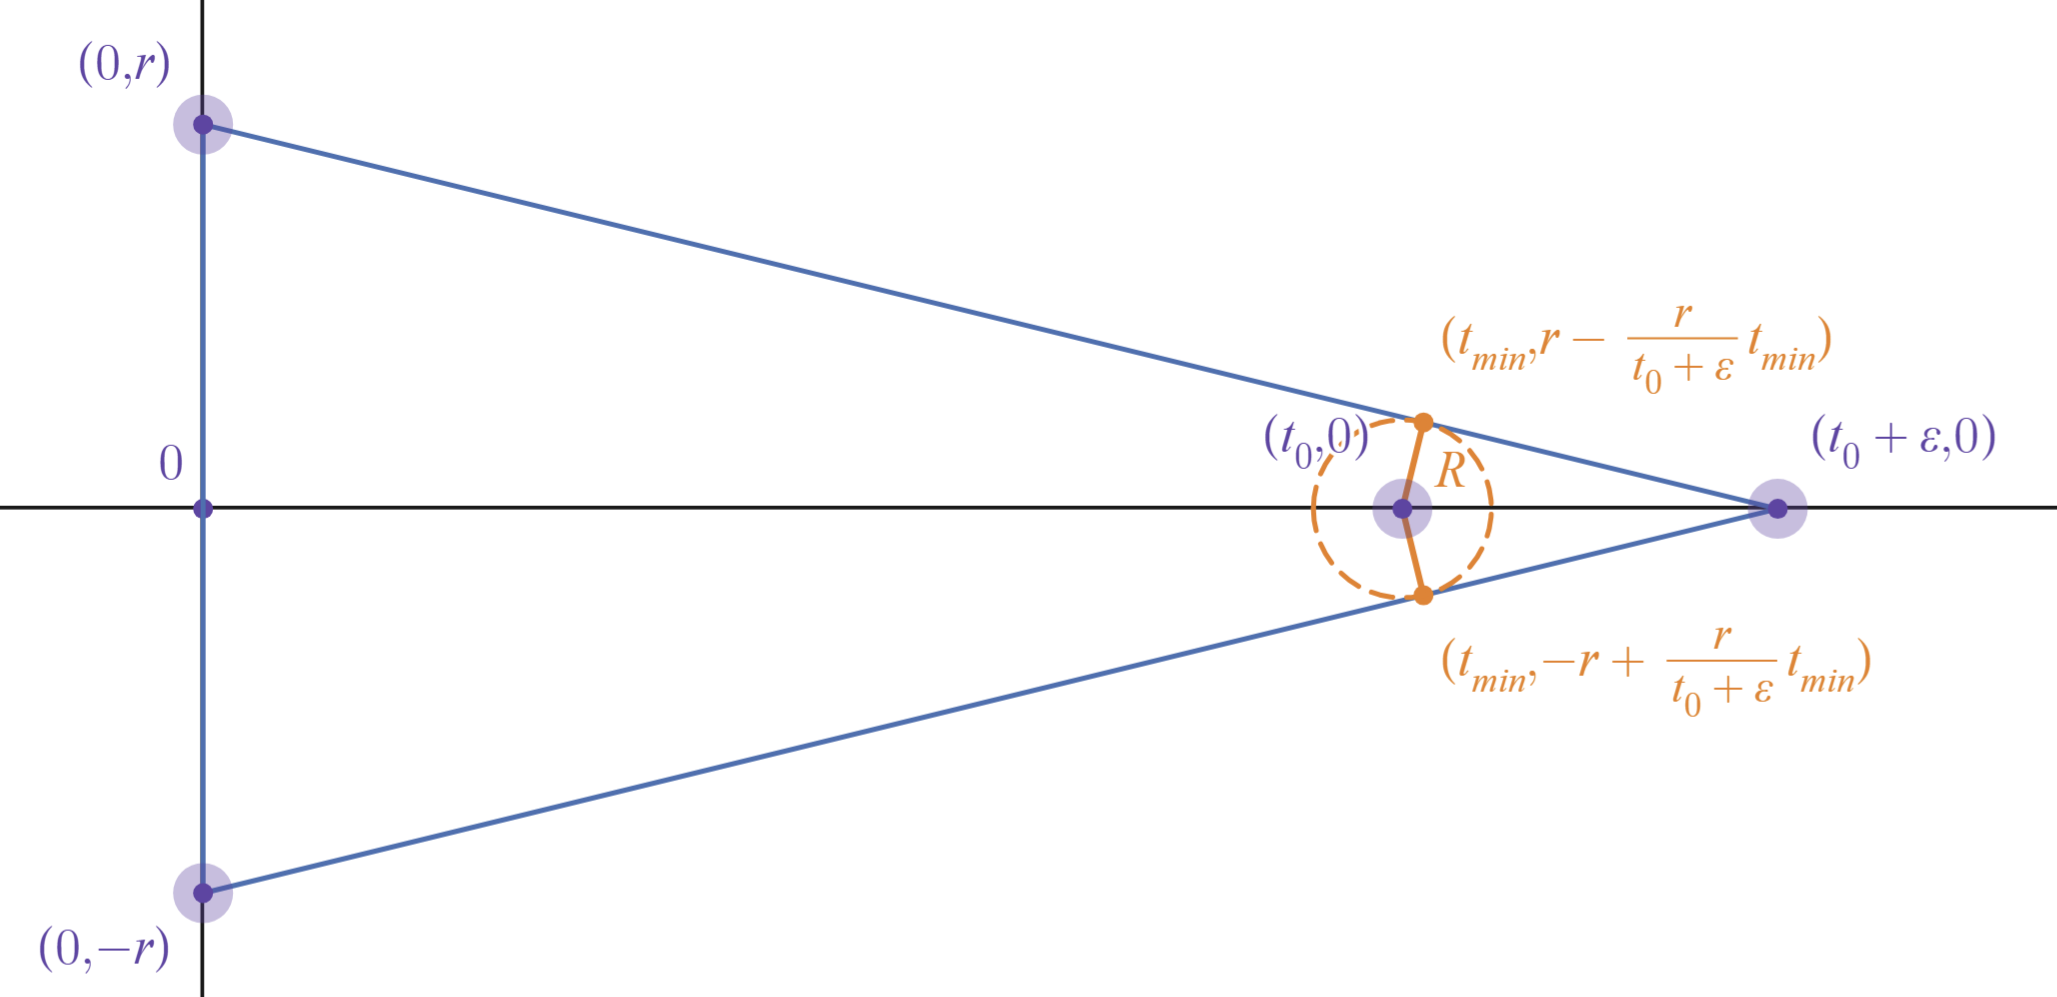
\includegraphics[scale=0.44]{Doing_Geometry_page_318.png}\par}
	\end{tabular}

	\newpage

	Since $X$ is closed (since it's compact) and thus includes it's boundary, we've now proven that if $f(t_0) \in \partial X$ then $f(t) \notin \partial X$ for all $t > t_0$. And hence, our ray can intercept $\partial X$ at most once. $\blacksquare$
	\begin{myIndent}\myComment
		As a side note: something even more fucked up is that the radius proposed by this paper doesn't work. It's too large. Anyways, because the paper handwaves this next bit, I'm going to deviate from the paper a bit.\retTwo
	\end{myIndent}
\end{myIndent}

\pracOne\mySepTwo
\ul{Lemma:} Let $\mathcalli{X}$ be a topological $K$-vector space where $K = \mathbb{R}$ or $\mathbb{C}$. Also suppose $E \subseteq X$ and $c \in K$. 
\begin{itemize}
	\item If $E$ is convex, then so is $cE$.
	\begin{myIndent}\pracTwo
		Proof:\\
		If $E$ is empty or $c = 0$, this is obvious. Otherwise, suppose $x, y \in cE$ and then note that $c^{-1}x, c^{-1}y \in E$. It follows that $c^{-1}(tx + (t-1)y) \in E$. So, $tx + (1-t)y \in cE$.\retTwo
	\end{myIndent}

	\item $c(\overline{E}) = \overline{cE}$.
	\begin{myIndent}\pracTwo
		Proof:\\
		If $c = 0$ then it must be the case that both sets are empty or are $\{0\}$. Meanwhile, note that as a general fact if $f : X \to Y$ is a continuous map and $A \subseteq X$, then $f^{-1}(\overline{f(A)})$ is a closed set containing $A$. Hence $\overline{A} \subseteq f^{-1}(\overline{f(A)})$ and this proves that $f(\overline{A}) \subseteq \overline{f(A)}$. Since scalar multiplication by $c$ is a homeomorphism of $\mathcalli{X}$ when $c \neq 0$, we thus have that $c\overline{E} = \overline{cE}$. $\blacksquare$\retTwo
	\end{myIndent}

	\item $c(\partial E) = \partial (cE)$.
	\begin{myIndent}\pracTwo
		Proof:\\
		By the last bullet point plus the fact that $f(A \cap B) = f(A) \cap f(B)$ for any function, we know that $c(\partial E) = c(\overline{E} \cap \overline{E^\comp}) = \overline{cE} \cap \overline{c(E^\comp)}$. Now if $c = 0$, then we know that $c(\partial E)$ and $\partial (cE)$ are either both empty or both $\{0\}$. So, we may assume that $c \neq 0$. But in that case scalar multiplication is a homeomorphism on $\mathcalli{X}$. So $c(E^\comp) = (cE)^\comp$ and we've shown that $c(\partial E) = \overline{cE} \cap \overline{(cE)^\comp} = \partial (cE)$.\retTwo
	\end{myIndent}
\end{itemize}

\ul{Lemma:} Suppose $f: X \to Y$ is a homeomorphism and $A, B \subseteq X$. (This would include the case that $X = Y = \mathcalli{X}$ and $f$ is scalar multiplication by a nonzero scalar). Then\\ $f(E^\circ) = (f(E))^\circ$.
\begin{myIndent}\pracTwo
	Proof:\\
	Since $f$ is continuous and bijective, $f^{-1}(f(A)^\circ)$ is an open set contained in $A$. So,\\ $f^{-1}(f(A)^\circ) \subseteq A^\circ$ and hence $f(A)^\circ \subseteq f(A^\circ)$. On the other hand, since $f^{-1}$ is\\ continuous, we know that $f(A^\circ)$ is an open subset of $f(A)$. So, $f(A^\circ) \subseteq f(A)^\circ$.\retTwo
\end{myIndent}

\mySepTwo

\exTwo\ul{Theorem:} Suppose $X \subseteq \mathbb{R}^n$ is a convex body and contains $0$. Then $X$ is homeomorphic to the closed unit ball $\overline{B_1(0)}$.

\begin{myIndent}\exThreeP
	Proof:\newpage
	Let $p_{X^\circ}$ be the Minkowski functional associated with $X^\circ$. In other words,\\ $p_{X^\circ}(x) = \inf \{t \geq 0 : x \in tX\}$. Unfortunately, since $X$ isn't a balanced set\\ necessarily, we can't directly apply the proof on \inLinkRap{Minkowski functional reference}{page 233} to get that $P_{X^\circ}(cx) = |c|x$\\ for all $c \in \mathbb{R}$ and $x \in \mathbb{R}^n$. That said, since $X$ is convex and a neighborhood of $0$, we are able to copy the reasoning that shows that $p_{X^\circ}$ is well-defined and satisfies the triangle inequality.\retTwo

	\ul{Claim 1:} Suppose $y$ is any unit vector and $t_0$ is the unique nonnegative number satisfying that $t_0 y \in \partial X$. Then $p_{X^\circ}(ty) = \sfrac{t}{t_0}$.
	\begin{myIndent}\exPPP
		Proof:\\
		If $t = 0$, then it is obvious that $p_{X^\circ}(ty) = 0 = \sfrac{t}{t_0}$. As for when $t \neq 0$, first note that $t_0 y \in \partial X \Longleftrightarrow bt_0 y \in \partial(bX)$ for all $b \geq 0$. Also note that $bX$ is easily checked to be convex body when $b \neq 0$ (and so we can apply theorem 3.6 to $bX$).\retTwo

		Suppose $b < \sfrac{t}{t_0}$. Then $bt_0 < t$ and thus $t \notin X$ since $bt_0 y \in \partial (bX)$. On the other hand, suppose $b > \sfrac{t}{t_0}$. Then $bt_0 > t$ and thus $t \in X - \partial X = X^\circ$ since again $bt_0 y \in \partial (bX)$. It follows that $p_{X^\circ}(ty) = \sfrac{t}{t_0}$.\retTwo
	\end{myIndent}

	\ul{Corollary:} Suppose $x \in X$ and $t_0 > 0$ is the unique nonnegative number such that\\ $t_0 \frac{x}{\|x\|_2} \in \partial X$. Then $p_{X^\circ}(x) = \sfrac{\|x\|_2}{t_0}$.\retTwo

	\ul{Claim 2:} $p_{X^\circ}$ is continuous.
	\begin{myIndent}\exPPP
		Proof:\\
		While we don't necessarily have reverse triangle inequality since $p_{X^\circ}(x) \neq p_{X^\circ}(-x)$, we can at least prove using just triangle inequality that:

		{\centering $|p_{X^\circ}(x) - p_{X^\circ}(y)| \leq \max(p_{X^\circ}(x - y), p_{X^\circ}(y - x))$ \retTwo\par}

		Then, you just need to follow almost identical reasoning to that of \inLinkRap{Minkowski functional reference}{page 233} to show that $p_{X^\circ}(x)$ is continuous.\retTwo
	\end{myIndent}

	At last we are ready to write our homeomorphism from $X$ to $B$. Define $g : X \to \overline{B_1(0)}$ by $g(x) = p_{X^\circ}(x)\frac{x}{\|x\|_2}$ when $x \neq 0$ and $g(0) = 0$. And similarly, define $h : \overline{B_1(0)} \to X$ by $h(y) = ty$ such that $ty \in \partial(\|y\|X)$.
	\begin{itemize}
		\item $g$ is continuous when $x \neq 0$ by virtue of being a scalar product of continuous\\ functions. Also, given any sequence $(x_n)_{n \in \mathbb{N}}$ in $X$ converging to $0$ we have that\\ $\|g(x_n)\|_2 = p_{X^\circ}(x_n) \cdot 1 \to 0$ as $n \to \infty$. So $g$ is also continuous at $0$.\retTwo
		
		\item $h(g(0)) = 0$. Meanwhile, suppose $x \in X - \{0\}$. Then let $t_0$ be the unique\\ [2pt] nonnegative number satisfying that $t_0 \frac{x}{\|x\|_2} \in \partial X$. Now $g(x) = p_{X^\circ}(x) \frac{x}{\|x\|_2} = \frac{x}{t_0}$.\\ [-1pt] Thus $h(g(x)) = t \frac{x}{t_0}$ where $t \geq 0$ satisfies that $t \frac{x}{t_0} \in \partial(\frac{\|x\|}{t_0}X)$. Or in other words,\\ [3pt] $t\frac{x}{\|x\|_2} \in \partial X$. It follows by theorem 3.6 that $t = t_0$ and so $h(g(x)) = x$.\retTwo
		
		\item $g(h(0)) = g(0) = 0$. Meanwhile, if $y \in \overline{B_1(0)} - \{0\}$ then let $t_0$ be the\\ unique nonnegative number such that $t_0 \frac{y}{\|y\|_2} \in \partial X$. Like before, we can show\\ that $h(y) = t_0 y$. And now $p_{X^\circ}(t_0 y) = \frac{t_0\|y\|_2}{t_0} = \|y\|_2$ since $t_0 y = t_0 \|y\|_2 \frac{y}{\|y\|_2}$.\\ Thus $g(t_0 y) = g(t_0 y) = \|y\|_2\frac{t_0y}{\|t_0y\|_2} = y$ and we've proven that $g(h(y)) = y$.\newpage
		
		\item Since $h = g^{-1}$, $g$ is continuous, $X$ is compact, and $\overline{B_1(0)}$ is Hausdorff, we have that $h$ is continuous. $\blacksquare$\retTwo
	\end{itemize}
\end{myIndent}

\ul{Corollary:} All convex bodies in $\mathbb{R}^n$ are homeomorphic to the closed unit ball $\overline{B_1(0)}$.
\begin{myIndent}\exThreeP
	Why? We can just translate them so that they contain $0$ and then apply the last theorem.\retTwo
\end{myIndent}

\ul{Corollary 2:} All $n$-simplices are homeomorphic to the closed unit ball $\overline{B_1(0)}$ in $\mathbb{R}^n$.\retTwo

\hTwo\mySepTwo 

\dispDate{10/18/2025}

I need to first do the rest of my math 200a homework. Then I think there is a different paper I want to try to following to prove the fixed point theorems from before.\retTwo

\blect{Math 200a Homework:}\retTwo

\Hstatement\blab{Set 3 Problem 3:} Suppose $G$ is a finite group and $h < G$. Suppose also for all $x \in H - \{1\}$ that $C_G(x) \subseteq H$. Then $\gcd(|H|, [G : H]) = 1$.
\begin{myIndent}\HexOne
	Proof:\\
	If $\gcd(|H|, [G : H]) \neq 1$, then we know there is some prime number $p$ dividing both $|H|$ and $[G : H]$. And as a result, $\nu_p(|H|) < \nu_p(|G|)$. So, by choosing $P \in \Syl_p(H)$ and $Q \in \Syl_p(G)$, we know that $|P| < |Q|$. Also, by Sylow's second theorem, we can conjugate $Q$ in order to say without loss of generality that $P \subseteq Q$. We'll need two observations:
	\begin{itemize}
		\item Since the order of $Q$ doesn't divide $H$, we know that $Q$ isn't a subgroup of $H$. Hence, $Q \cap (G - H) \neq \emptyset$.
		\item At the same time though, we know that $P < Q \cap H < H$. And since the only prime factors of $|Q \cap H|$ are $p$, this tells us by Lagrange's theorem that $|P| = p^{\nu_p(|H|)}$ divides $|Q \cap H|$ which itself divides $p^{\nu_p(|H|)}$. Hence, $|P| = |Q \cap H|$ and this proves that $Q \cap H = P$. \retTwo
	\end{itemize}

	Now recall from the 2nd proposition on \inLinkRap{Alireza theorem center of p groups}{page 272} that if $\{1\} \neq N \lhd P$ and $P$ is a $p$-group, then $Z(P) \cap N \neq \{1\}$.
	\begin{myIndent}\exPPP
		Side note: Whenever $H < G$, we define $Z(H) = \bigcap_{h \in H}C_H(h)$. Just wanted to make that's clear since I didn't know better before.\retTwo
	\end{myIndent}

	As a special case, if we set $N = P$ (where $P$ is nontrivial), then this proposition says that the center of a $p$-group is always nontrivial. Hence, there exists $y \in Z(P) - \{1\}$.
	\begin{myIndent}\exPPP
		Side note: How the hell hadn't I processed that consequence of the theorem we\\ proved before?\retTwo
	\end{myIndent}

	Now note that $Z(Q) \subseteq C_Q(y) \subseteq C_G(y) \subseteq H$ where the last inclusion is by the\\ assumption of the problem. Hence $Z(Q) \subseteq H \cap Q = P$. At the same time, we know\\ that $Z(Q)$ is nontrivial. So, there exists $x \in Z(Q) - \{1\}$ which we know from before is\\ in $P \subseteq H$. Finally, we now have that $Q \subseteq C_Q(x) \subseteq C_G(x) \subseteq H$. But this contradicts that $Q \cap (G - H) \neq \emptyset$. $\blacksquare$\retTwo
\end{myIndent}

\blab{Set 3 Problem 8:} Suppose $G$ is a finite group.
\begin{enumerate}
	\item[(a)] Prove that a normal Sylow $p$-subgroup is a characteristic subgroup.\newpage
	
	\begin{myIndent}\HexOne
		A Sylow $p$-subgroup $P$ is normal if and only if it is the only Sylow $p$-subgroup. And since automorphisms preserve the order of subgroups, we have that if $P$ is the only subgroup of $G$ with order $p^{\nu_p(|G|)}$ then $\theta(P) = P$ for all $\theta \in \Aut(G)$. So, $P$ is a characteristic subgroup.\retTwo
	\end{myIndent}
	
	\item[(b)] Suppose $H \lhd G$ and $\gcd(|H|, [G : H]) = 1$. Prove that $H$ is a characteristic subgroup.
	
	\begin{myIndent}\HexOne
		Suppose $\theta \in \Aut(G)$. Then since $H$ is normal, we know that $\theta(H)H$ is a subgroup of $G$ and $H \lhd \theta(H)H$. So by the correspondance theorem, we know that $|\frac{\theta(H)H}{H}|$ divides $|G/H| = [G : H]$. At the same time, $|\theta(H)H| = \frac{|H||\theta(H)|}{|H \cap \theta(H)}$. So, $|\frac{\theta(H)H}{H}| = \frac{|\theta(H)|}{|H \cap \theta(H)}$ divides $|\theta(H)| = |H|$.\retTwo

		This shows that $|\frac{\theta(H)H}{H}| \divides \gcd(|H|, [G : H]) = 1$. And hence, $\theta(H)H = H$. Since $|\theta(H)| = |H|$ and $\theta(H) \subseteq \theta(H)H$, we can thus conclude that $\theta(H) = H$. $\blacksquare$\retTwo
	\end{myIndent}
\end{enumerate}

\blab{Set 3 Problem 4:} Suppose $G$ is a finite group, $N \lhd G$, and $p$ is a prime factor of $|N|$.
\begin{myIndent}
	\item[(a)] Suppose $P \in \Syl_p(G)$ and $Q \in \Syl_p(N)$. Prove there exists $g \in G$ such that\\ $Q = (gPg^{-1}) \cap N$.
	
	\begin{myIndent}\HexOne
		Uhhhh, I think I already basically proved this fact when doing problem 3.\retTwo

		By Sylow's second theorem, we know there is some $g \in G$ such that $Q \subseteq gPg^{-1}$. Then since $(gPg^{-1}) \cap N$ is a subgroup of $gPg^{-1}$ where the latter is a $p$-group, we know that $(gPg^{-1}) \cap N$ is also a $p$-group. Also, since $(gPg^{-1}) \cap N$ is a subgroup of $N$, we know that $|(gPg^{-1}) \cap N|$ divides $|N|$. It follows that $|(gPg^{-1}) \cap N|$ divides $p^{\nu_p(|N|)}$. At the same time, since $|Q| = p^{\nu_p(|N|)}$ and $Q \subseteq gPg^{-1} \cap N$, we have that $p^{\nu_p(|N|)} \leq |(gPg^{-1}) \cap N|$.\retTwo

		So, $Q \subseteq (gPg^{-1}) \cap N$ and $|Q| = p^{\nu_p(|N|)} = |(gPg^{-1}) \cap N|$. It follows that\\ $Q = (gPg^{-1}) \cap N$.
		\begin{myIndent}\myComment
			Side note: none of the reasoning in this part requires having $N$ be normal.\retTwo
		\end{myIndent}
	\end{myIndent}
	
	\item[(b)] Prove that the following is a well-defined surjective function:
	
	{\centering $\Phi : \Syl_p(G) \to \Syl_p(N)$ where $\Phi(P) = P \cap N$. \retTwo\par}

	\begin{myIndent}\HexOne
		Part (a) guarentees that the above map will be surjective provided that it is well-\\defined (since $gPg^{-1} \in \Syl_p(G)$ for any $P \in \Syl_p(G)$). Hence, all we need to show\\ is that $P \cap N \in \Syl_p(N)$ whenever $P \in \Syl_p(G)$.\retTwo

		Fortunately since $P \cap N < P$, we know that $P \cap N$ is a $p$-group. But suppose for\\ the sake contradiction that $|P \cap N| \neq p^{\nu_p(|N|)}$ (meaning $P \cap N \notin \Syl_p(G)$). Then,\\ by Sylow's first and second theorems there exists a group $Q \in \Syl_p(N)$ such that\\ $P \cap N \lneqq Q < N$. Also, by part (a) there exists $g \in G$ such that $Q = gPg^{-1} \cap N$. But since $N$ is normal, $gPg^{-1} \cap N = gPg^{-1} \cap gNg^{-1} = g(P \cap N)g^{-1}$.
		\begin{myIndent}\HexPPP
			The last equality is obvious if you think about it. So I'd rather not write out a proof since I want to go on an outing soon.\retTwo
		\end{myIndent}

		So $P \cap N \lneqq Q = g(P \cap N)g^{-1}$. Since $|P \cap N| = |g(P \cap N)g^{-1}|$ this is a contradiction.\newpage
	\end{myIndent}

	\item[(c)] For $P \in \Syl_p(G)$, prove that $N_G(P) \subseteq N_G(\Phi(P))$ and:
	
	{\centering $|\Phi^{-1}(\Phi(P))| = [N_G(\Phi(P)) : N_G(P)]$. \retTwo\par}

	\begin{myIndent}\HexOne
		To start off, note that:
		
		{\centering\begin{tabular}{l}
			$\Phi(xPx^{-1}) = xPx^{-1} \cap N = xPx^{-1} \cap xNx^{-1}$\\
			$\phantom{\Phi(xPx^{-1}) = xPx^{-1} \cap N} = x(P \cap N)x^{-1} = x\Phi(P)x^{-1}$.
		\end{tabular}\retTwo\par}

		Therefore, if $x \in N_G(P)$ then $\Phi(P) = \Phi(xPx^{-1}) = x\Phi(P)x^{-1}$. And this proves the first claim that $N_G(P) \subseteq N_G(\Phi(P))$.\retTwo

		Next, note by Sylow's second theorem that:
		
		{\centering$\Phi^{-1}(\Phi(P)) = \{gPg^{-1} : g \in G \text{ and } \Phi(P) \subseteq gPg^{-1}\}$.\retTwo\par}

		But $\Phi(P) \subseteq gPg^{-1}$ if and only if:
		
		{\centering\begin{tabular}{l}
			$\Phi(P) = P \cap N \subseteq gPg^{-1} \cap N = (gPg^{-1}) \cap (gNg^{-1})$\\
			$\phantom{\Phi(P) = P \cap N \subseteq gPg^{-1} \cap N} = g(P \cap N)g^{-1} = g\Phi(P)g^{-1}$.
		\end{tabular}\retTwo\par}

		And since $|\Phi(P)| = |g\Phi(P)g^{-1}|$, this is the same as saying that $\Phi(P) = g\Phi(P)g^{-1}$. So, we really have that:

		{\centering$\Phi^{-1}(\Phi(P)) = \{gPg^{-1} : g \in N_G(\Phi(G))\}$.\retTwo\par}

		Hence, if we consider the action $N_G(\Phi(P)) \curvearrowright \Syl_p(G)$ by conjugation, then\\ [-1pt] $\Phi^{-1}(\Phi(P))$ is precisely the orbit of $P$ with respect to this action. Also, $x$ is in the stabilizer of $P$ with respect to this action precisely when $xPx^{-1} = P$. Or in other\\ words, $x \in (N_G(\Phi(P)))_P$ when $x \in N_G(\Phi(P)) \cap N_G(P) = N_G(P)$. By the\\ orbit-stabilizer theorem, we thus can conclude that:
		
		{\centering$|\Phi^{-1}(\Phi(P))| = [N_G(\Phi(P)) : N_G(P)]$.\retTwo\par}
	\end{myIndent}

	\item[(d)] Prove that $|\Syl_p(N)|$ divides $|\Syl_p(G)|$.
	
	\begin{myIndent}\HexOne
		We know that $\{\Phi^{-1}(Q) : Q \in \Syl_p(N)\}$ forms a partion of $\Syl_p(G)$. Hence, we\\ [-2pt] now seek to prove that there exists a single integer $r \in \mathbb{N}$ such that $|\Phi^{-1}(Q)| = r$ for all $Q \in \Syl_p(N)$. After all, once we know that we will then be able to say that $\Syl_p(N) = r \Syl_p(G)$.\retTwo

		Luckily, note that since conjugation is an automorphism of $G$ we have that:
		\begin{itemize}
			\item $|N_G(P)| = |g(N_G(P))g^{-1}| = |(N_G(gPg^{-1}))|$,
			\item $|N_G(\Phi(P))| = |g(N_G(\Phi(P)))g^{-1}| = |N_G(g\Phi(P)g^{-1})| = |N_G(\Phi(gPg^{-1}))|$.\retTwo
		\end{itemize}

		It follows for all $g \in G$ and $P \in \Syl_p(G)$ that:

		{\centering\begin{tabular}{l}
			$|\Phi^{-1}(\Phi(P))| = [N_G(\Phi(P)) : N_G(P)]$ \\ [4pt]
			$\phantom{|\Phi^{-1}(\Phi(P))|} = \frac{|N_G(\Phi(P))|}{|N_G(P)|} = \frac{|N_G(\Phi(gPg^{-1}))|}{|N_G(gPg^{-1})|} = [N_G(\Phi(gPg^{-1})) : N_G(gPg^{-1})]$\\
			$\phantom{|\Phi^{-1}(\Phi(P))| = \frac{|N_G(\Phi(P))|}{|N_G(P)|} = \frac{|N_G(\Phi(gPg^{-1}))|}{|N_G(gPg^{-1})|}} = |\Phi^{-1}(\Phi(gPg^{-1}))|$
		\end{tabular}\retTwo\par}

		And since $G$ acts transitively on $\Syl_p(G)$ by conjugation, this means that there exists\\ $r \in \mathbb{N}$ such that $r = |\Phi^{-1}(\Phi(P))|$ for all $P \in \Syl_p(G)$. And since $\Phi$ is surjective,\\ we have that $\Phi^{-1}(Q) = r$ for all $Q \in \Syl_p(G)$. $\blacksquare$\retTwo
	\end{myIndent}
\end{myIndent}



% ~~~~~~~~~~~~~~~~~~~~~~~~~~~~~~~~~~~~~~~~~~~~~~
\hypertarget{bib citation 17}{}

\hypertarget{Minkowski functional reference}{}



\hypertarget{Ergodic reading group notes 3}{}

\hypertarget{existence and uniqueness diff eq notes}{}

\hypertarget{page 251 reference}{}
\hypertarget{page 271 reference}{}
\hypertarget{page 270 reference}{}
\hypertarget{Alireza theorem page 271}{}
\hypertarget{Cauchy's theorem page 271}{}
\hypertarget{Alireza theorem center of p groups}{}

\hypertarget{math 241a lecture 5}{}
\hypertarget{math 200a lecture 9}{}
\hypertarget{math 220a lecture 9}{}


\hypertarget{page 284 reference example 1.2.1}{}

\hypertarget{idk reference 2}{}

\hypertarget{math 220a theorem II.2.3}{}
\hypertarget{Cauchy-Riemann equations theorem}{}



\end{document}



% \hTwo Suppose $|G| = pq$ where $p < q$ are prime numbers. Then $s_q = 1$. Hence there exists a unique Sylow $q$-subgroup $Q$. Furthermore, $Q \lhd G$ and $Q$ is cylic with order $q$.\retTwo

% Next, let $P$ by a Sylow $p$-subgroup. Then because $Q \lhd G$, we have that $PQ < G$. Also, $|P \cap Q| \divides \gcd(p, q) = 1$. So, $P \cap Q = \{1\}$ and from there it follows that $|PQ| = pq = |G|$. So $G / Q = PQ / Q \cong P / (P \cap Q) \cong P$.

